\section{Quickstart}

\subsection{Accessing the server}

You can access UniNuvola via web browser, using the University VPN, through the
\href{https://www.uninuvola.unipg.it/}{https://www.uninuvola.unipg.it/} website. You will be redirected to the UniNuvola
Vault login page. After selecting the LDAP option (Figure \ref{fig:login}) in the drop-down menu, you can enter your
login details: these are the same as those you use to access the University services (user id and password).

\begin{figure}[!ht]
    \centering
    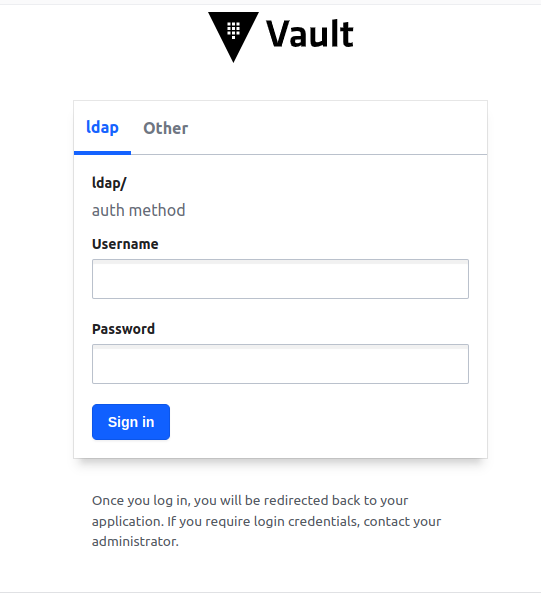
\includegraphics[width=0.5\linewidth]{img/login_page.png}
    \caption{UniNuvola's login page.}
    \label{fig:login}
\end{figure}

\subsubsection{First time access }
If it is your first time accessing the server, you will be redirected to a web page  where you will automatically request access to the infrastructure. Access will be granted once one of the operators approves your request (Figure
\ref{fig:pending}).
\begin{figure}[!ht]
    \centering
    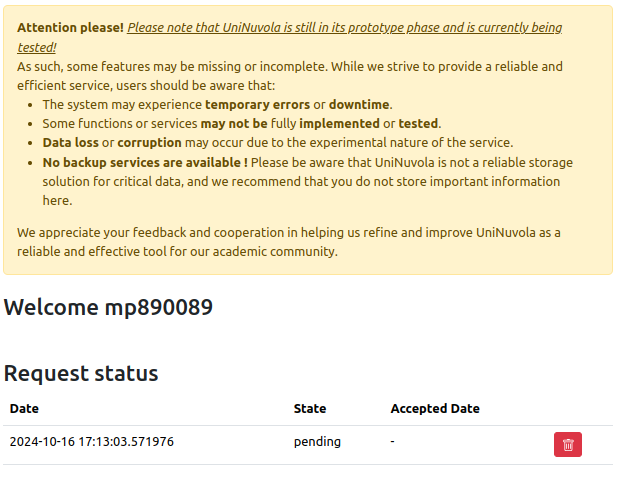
\includegraphics[width=0.5\linewidth]{img/request_page.png}
    \caption{Pending acceptance page}
    \label{fig:pending}
\end{figure}

\subsubsection{Following accesses.}
Once you get accepted, after login into Vault, you will be redirected the  starting page, where you can choose the image and resources.

\begin{bclogo}[logo=\bcinfo, couleurBarre=orange, noborder=true, couleur=white]{Warning}
If you didn't logout after your account creation, or your token expired, it is possible that in the following session
you can be readdressed into the login page.  In order to solve the issue you can opt for two solutions:  disconnect by hand from the \href{https://vault.uninuvola.unipg.it:8200/ui/vault/dashboard}{UniNuvola Vault webpage}, or delete the cookies in your browser.

\end{bclogo}


\subsection{Selection of the Image and resources}

After a successful login, you will be directed to the resource selection page. The first section to complete is the
image selection. This part needs to be filled in by the user or select one of the available options. Images can be
selected from those available in UniNuvola (see table \ref{tab:images}) or from your own customised version on
Dockerhub or quay.io. The tags \textit{latest} and \textit{main} are the official versions available in our repositories. The \textit{main} tag corresponds to the recommended image version for users to use; the \textit{latest} tag  corresponds to working version of the image, that is being tested before moving it to the \textit{main} tag.\\

%\begin{table}[]
%    \caption{List of the official images in UniNuvola}
%    \label{tab:images}
%    \centering
%    \begin{tabular}{|c|c|}
%        \hline
%        Base              & harbor1.fisgeo.unipg.it/uninuvola/base             \\ \hline
%        Engineering       & harbor1.fisgeo.unipg.it/uninuvola/engineering      \\ \hline
%        Conda             & harbor1.fisgeo.unipg.it/uninuvola/conda            \\ \hline
%        Chemistry         & harbor1.fisgeo.unipg.it/uninuvola/chemistry        \\ \hline
%        Quantum Computing & harbor1.fisgeo.unipg.it/uninuvola/quantumcomputing \\ \hline
%        Genomics          & harbor1.fisgeo.unipg.it/uninuvola/genomics         \\ \hline
%        Hydraulics        & harbor1.fisgeo.unipg.it/uninuvola/hydraulics       \\ \hline
%        Tensorflow        & harbor1.fisgeo.unipg.it/uninuvola/tensorflow       \\ \hline
%        Pytorch           & harbor1.fisgeo.unipg.it/uninuvola/pytorch          \\ \hline
%        Pytorch-GPU       & harbor1.fisgeo.unipg.it/uninuvola/pytorchgpu       \\ \hline
%        Optimisation      & harbor1.fisgeo.unipg.it/uninuvola/optimisation     \\ \hline
%    \end{tabular}
%\end{table}


The image name will appear as:
\begin{lstlisting}[language=bash] 
harbor1.fisgeo.unipg.it/uninuvola/base:main
\end{lstlisting}

In the next drop-down menus, you will choose the required resources, as it is shown in Figure \ref{fig:resources}.\\

\begin{figure}[!ht]
    \centering
    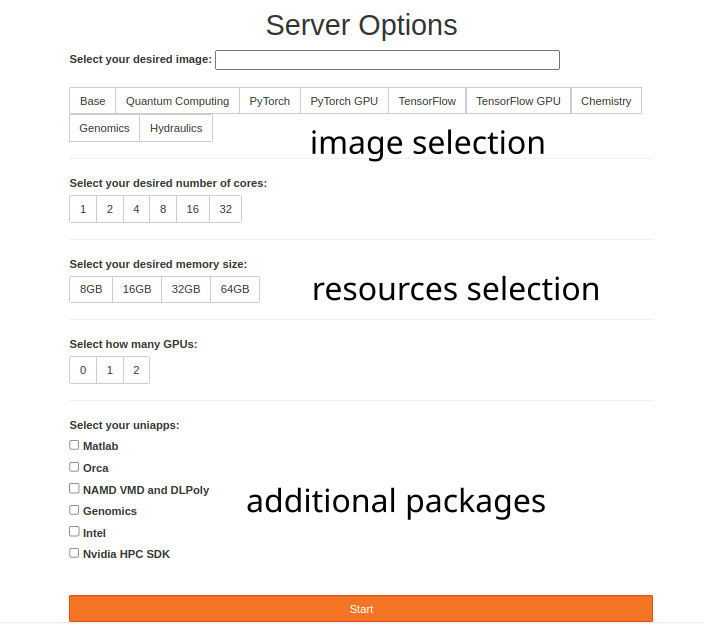
\includegraphics[width=0.75\linewidth]{img/resource_selection.png}
    \caption{Resources selection page}
    \label{fig:resources}
\end{figure}

As per the disclaimer in Figure \ref{fig:pending}, remember: \textbf{UniNuvola is a prototype. We provide computational
    power and storage, but data are not backed up. Be careful with your data!} \\

\subsection{Inside UniNuvola}
The main page of UniNuvola appears as depicted in Figure \ref{fig:uninuvola_main_page}. The top bar allows some
management actions and some customisation of the user interface. Most importantly, inside the file men, you can find the
disconnect and  the control hub options. The former allows to connect and disconnect from Jupyter (be aware that you
will disconnect from the Hub page, but the pod will continue run up to 24 hours after becoming inactive), the later
option allows to kill the running image and it allows the user to load a new image. \\

The left side of the menu allows the management of the local files. The four most upper options allow the user in order
to: open new launchers tabs, create new directories, upload files, and refresh the browser. Files can be moved through
the web interface or through remote terminal connection from UniNuvola to the machine hosting the files. You can access multiple tabs in your notebook.\\ 

Inside the red rectangle in the left side, you can find some tools for managing processes: the running terminal and kernels, the table of contents that shows headings in notebooks and supported files, and the PYPI manager, that consents to check the installed plugins. \\ 

The orange square includes all Python and R toolkits. The top part includes all the environments notebooks in the image,
the bottom part instead the relative consoles. The top right part, the purple square, contains the Xpra notebook, that
allows the usage of programs requiring a graphical interface.  \\

In the last line, the first element, circled in green, allows the user to use a terminal. All terminals will start with
the bash terminal depending on the image. The elements circled in blue are the text editors in the Hub,  in the case
of the figure a general text editor, a Markdown and a Python file editor. \\

The purple square shows the virtual desktop environment inside UniNuvola. The latter is a quick responsive desktop that allows the user to access to GUI programs, as MATLAB, VSCodium ad Firefox. \\

\begin{figure}[!ht]
    \centering
    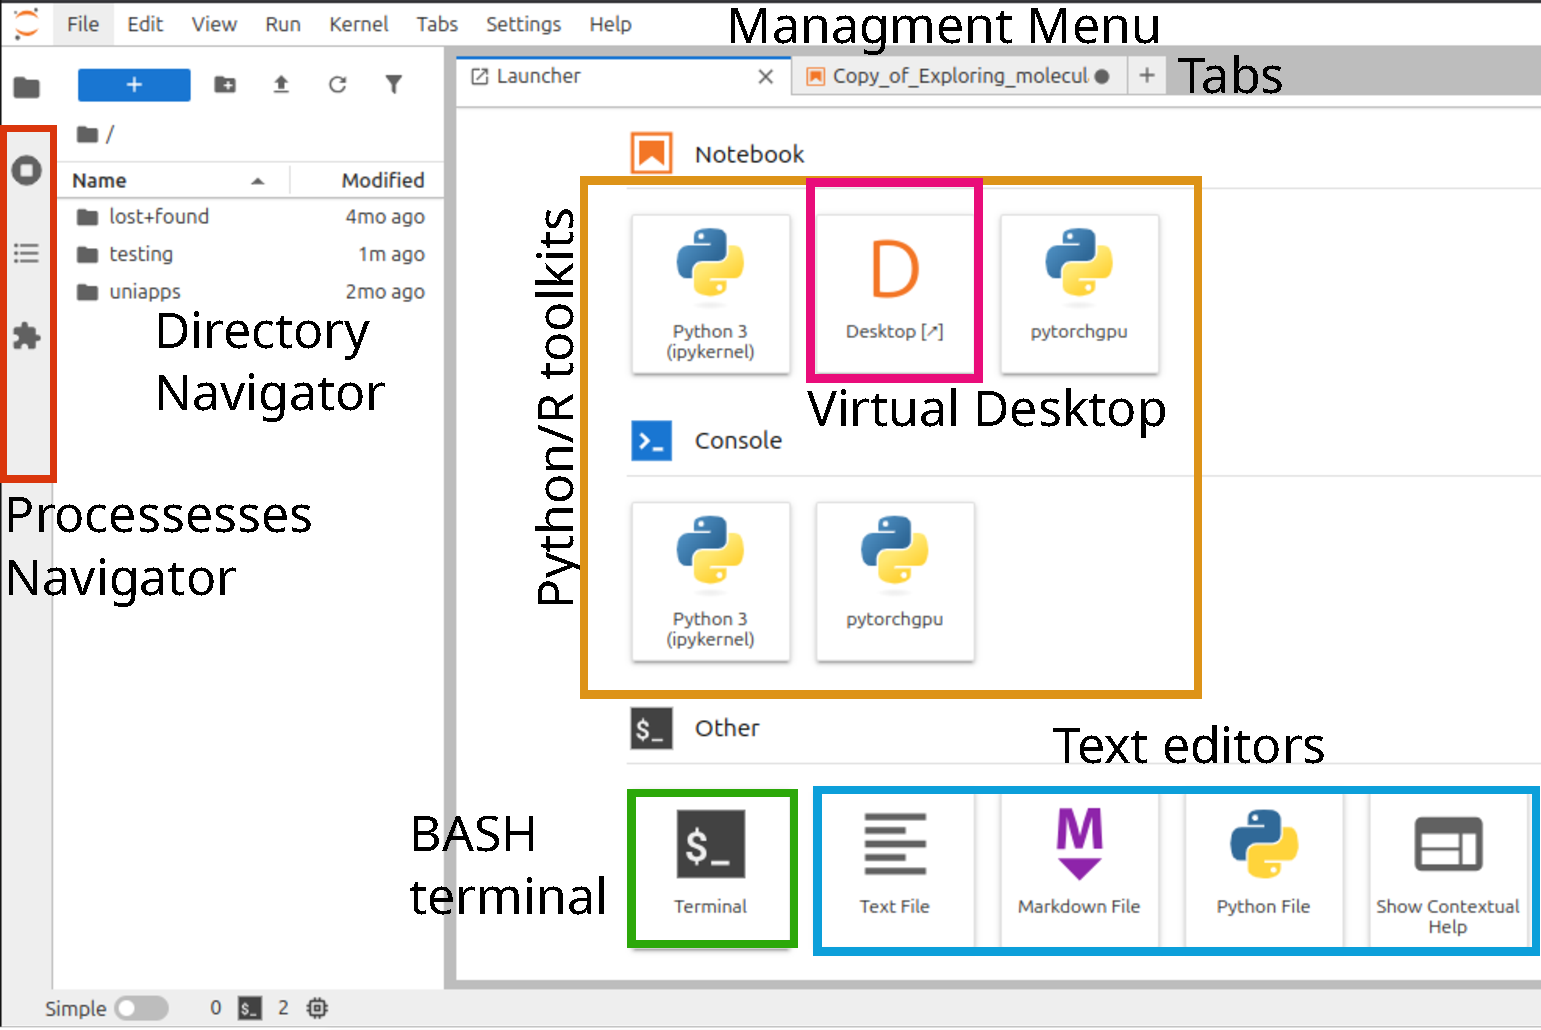
\includegraphics[width=0.8\linewidth]{img/uninuvola.pdf}
    \caption{Example of Jupyter Lab interface in UniNuvola.}
    \label{fig:uninuvola_main_page}
\end{figure}

\begin{figure}[!h]
    \center
    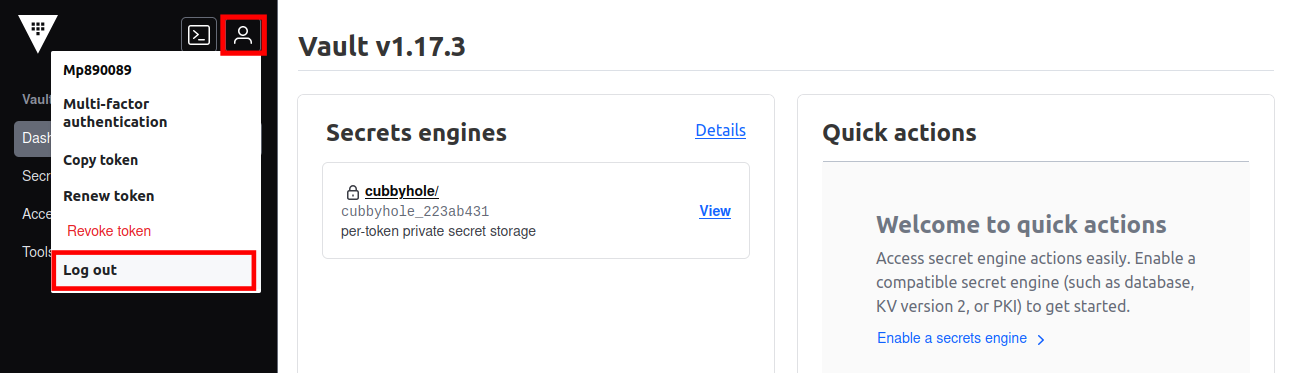
\includegraphics[width=0.8\linewidth]{img/vault.png}
    \caption{Uninvola's Vault logout page.}
    \label{img:logout}
\end{figure}
